\problemname{The Line}

Current urban planning is flawed.
Many busses and trams are needed to support a public transportation network.
What if we were to build an entire city along a line?
Then, the entire city's transportation needs could be met with a few high-speed trains.
With this brilliant idea, a city with $N$ train stations was built, each indexed between $1$ and $N$.
For every train station $i$ with $1 \leq i < N$, there is a train line to train station $i+1$, which takes $1$ minute.
Each line can be taken in both directions.

After a couple of years, it turns out that the shape of the city might not be optimal.
Thankfully, due to the prosperity of the city, you have developed a teleporter.
You are going to install the first teleporter and want to maximize its impact.
If you install the teleporter between train stations $i$ and $j$, you can teleport between the train stations in both directions.
Teleporting takes one minute.
There are $K$ people in the city.
Person $i$ lives in train station $s_i$ and works in train station $t_i$.
Let $\text{dist}(s,t)$ be the number of minutes that the shortest possible path between $s$ and $t$ takes,
which may or may not use the teleporter.

If you install the teleporter optimally, what is the minimum possible value of

$$\sum_{i=1}^{K} \text{dist}(s_i, t_i)$$

\section*{Input}

The first line contains two integers $N$ and $K$ ($1 \leq N \leq 10^9$, $1 \leq K \leq 10{,}000$),
the number of train stations and the number of people.

The following $K$ lines each contain two integers $s$ and $t$ ($1 \leq s,t \leq N$),
meaning that there is a person who lives at train station $s$ and works at train station $t$.
It is \textbf{not} guaranteed that all pairs ($s,t$) are unique.

\section*{Output}
Print an integer: the smallest total travel time if the teleporter is installed optimally.

\section*{Scoring}
Your solution will be tested on a set of test groups.
To earn points for a group, you must pass all test cases in that group.

\noindent
\begin{tabular}{| l | l | p{12cm} |}
  \hline
  \textbf{Group} & \textbf{Points} & \textbf{Constraints} \\ \hline
  $1$    & $7$         & $N, K \leq 50$ \\ \hline
  $2$    & $14$        & $N, K \leq 500$ \\ \hline
  $3$    & $27$        & $N, K \leq 2000$ \\ \hline
  $4$    & $13$        & $N \leq 2 \cdot 10^5, K \leq 500$  \\ \hline
  $5$    & $18$        & $N \leq 2 \cdot 10^5, K \leq 2000$  \\ \hline
  $6$    & $21$        & No additional constraints.  \\ \hline
\end{tabular}

\section*{Explanation of Samples}
In sample $1$, it is optimal to build the teleporter such that the single inhabitant can go work in one minute.

In sample $2$, one optimal solution is to build the teleporter between train stations $2$ and $9$.
In the drawing, every person's home is connected with their place of work,
and the optimal teleporter is drawn as a dotted line.

\begin{figure}[h]
  \centering
  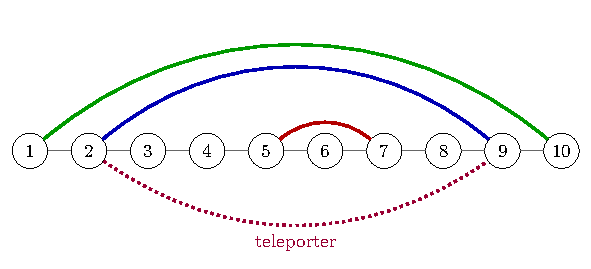
\includegraphics[width=0.7\textwidth]{sample2.pdf}
\end{figure}

The person who lives at train station $1$ takes the path $1 \rightarrow 2 \rightarrow 9 \rightarrow 10$,
the person at $2$ takes $2 \rightarrow 9$,
and the person at $5$ takes $5 \rightarrow 6 \rightarrow 7$.
In total, this takes $3+1+2=6$ minutes, which is optimal.

In sample $3$, one optimal solution is to build a teleporter between train stations $2$ and $9$.
